%{- block documentheader %}
%{- if fontsize %}
\documentclass[%{{-fontsize-%}}]{article}
%{- else %}
\documentclass[12pt]{article}
%{- endif %}

% colors
\usepackage[usenames,dvipsnames]{xcolor}

% FONT setup
\usepackage{lmodern}
\renewcommand\familydefault{\sfdefault}
\usepackage[utf8]{inputenc}
\usepackage[T1]{fontenc}

\usepackage{tikz}
\usetikzlibrary{positioning}
% set styling for tikz nodes used throughout document
\tikzset{% 
    default picture/.style={%
        font=\normalsize, node distance=0em, outer sep=0em, inner sep=0em
    },
    default line/.style={%
        black!100, solid, thick
    },
    full width text/.style={%
        minimum height=1em, minimum width=7.2in, text width=7.2in, align=left
    }
}

\usepackage{enumitem}
% set style for lists
\setlist[itemize]{itemsep=0pt, partopsep=0pt, topsep=0pt, label=$-$, leftmargin=*}

\usepackage{calc}
\usepackage[paper=letterpaper, includefoot,
            top=0.5in, bottom=0.5in, 
            left=0.65in, right=0.65in]{geometry}

\setlength{\parindent}{0in}

% header, footer setup
\usepackage{fancyhdr,lastpage}
\pagestyle{fancy} 
\fancyhead{}
\fancyfoot{}
\fancyfoot[]{}
\renewcommand{\headrulewidth}{0pt}
\renewcommand{\footrulewidth}{0pt}

% PDF
\usepackage{hyperref}
\hypersetup{
pdfstartview={FitH},
pdftitle={ Cover Letter :: %{{contact.name %}} },
pdfauthor={ %{{contact.name %}} },
pdfsubject={Resume for %{{ contact.name %}}},
pdfcreator={pdflatex, resumepy},
pdfproducer={pdflatex, resumepy},
colorlinks=true,
linkcolor=Black,
urlcolor=Black
%linkcolor=Mahogany,
%urlcolor=Mahogany
}
%{- endblock documentheader %}

\begin{document}

%{ block contact -%}

\textbf{ %{{- contact.name | escape_tex -%}} }
\hfill \textbf{web:} \href{http://%{{- website.label | escape_tex -%}} }{ %{{- website.link | escape_tex -%}} }

\vskip-0.75em
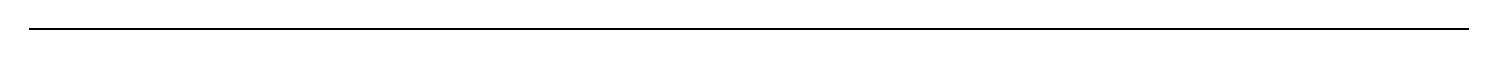
\begin{tikzpicture}[default picture]
\draw[default line] (0in, 0) -- (7.2in, 0);
\end{tikzpicture}

%{{contact.address | escape_tex -%}}, %{{ contact.city %}}, %{{contact.state %}} %{{ contact.zip %}} \\
\textbf{tel:} %{{ contact.phone %}} \textbf{email:} \href{mailto:%{{- contact.email -%}} }{ %{{- contact.email -%}} }
%{- endblock contact %}

%{ block company -%}
\vskip2em
%{ if company.contact -%} %{{ company.contact | escape_tex -%}} \\ %{- endif %}
%{ if company.jobtitle -%} %{{ company.jobtitle | escape_tex -%}} \\ %{- endif %}
%{{ company.name | escape_tex -%}} \\
%{{ company.address | escape_tex %}} \\
%{{ contact.city %}}, %{{ contact.state %}} %{{ contact.zip %}}
%{- endblock company %}

%{ block open -%}
\vskip2em
\today
\vskip2em
%{{ salutation | escape_tex %}}
%{- endblock open -%}

%{ block letter -%}
\vskip2em
\begin{tikzpicture}[default picture]
\node[full width text] at (0in, 0in) { %{{ letter | escape_tex | wordwrap %}} };
\end{tikzpicture}
%{- endblock letter %}

%{ block close -%}
%{ if signature %}
\vskip2em
%{{ closing | escape_tex %}}
\vskip1em
\pgfdeclareimage[]{signature}{ %{{- signature -%}} }
\scalebox{0.4}{
\begin{tikzpicture}
  \pgftext[at=\pgfpoint{0cm}{0cm},left,base]{\pgfuseimage{signature}}
\end{tikzpicture}  
}% end scalebox
\vskip1em
%{{- contact.name %}}
%{ else %}
\vskip2em
%{{ closing %}}
\vskip5em
%{{- contact.name %}}

%{ endif %}
%{- endblock close -%}

%%
%%
\end{document}
